% Created 2018-04-17 mar 13:49
% Intended LaTeX compiler: pdflatex
\documentclass[xcolor={usenames,svgnames,dvipsnames}]{beamer}
\usepackage[utf8]{inputenc}
\usepackage[T1]{fontenc}
\usepackage{graphicx}
\usepackage{grffile}
\usepackage{longtable}
\usepackage{wrapfig}
\usepackage{rotating}
\usepackage[normalem]{ulem}
\usepackage{amsmath}
\usepackage{textcomp}
\usepackage{amssymb}
\usepackage{capt-of}
\usepackage{hyperref}
\usepackage{color}
\usepackage{listings}
\usepackage{mathpazo}
\usepackage{gensymb}
\usepackage{amsmath}
\usepackage{chemarr}%flechas para reacciones químicas (SFER.tex)
\bibliographystyle{plain}
\AtBeginSubsection[]{\begin{frame}[plain]\tableofcontents[currentsubsection,sectionstyle=show/shaded,subsectionstyle=show/shaded/hide]\end{frame}}
\AtBeginSection[]{\begin{frame}[plain]\tableofcontents[currentsection,hideallsubsections]\end{frame}}
\usepackage[emulate=units]{siunitx}
\sisetup{fraction=nice, decimalsymbol=comma, retain-unity-mantissa = false}
\newunit{\wattpeak}{Wp}
\newunit{\watthour}{Wh}
\newunit{\amperehour}{Ah}
\hypersetup{colorlinks=true, linkcolor=Blue, urlcolor=Blue}
\renewcommand{\thefootnote}{\fnsymbol{footnote}}
\beamertemplatenavigationsymbolsempty
\setbeamertemplate{footline}[frame number]
\setbeamercolor{alerted text}{fg=blue!50!black} \setbeamerfont{alerted text}{series=\bfseries}
\usetheme[hideothersubsections]{Goettingen}
\usecolortheme{rose}
\usefonttheme{serif}
\author{Oscar Perpiñán Lamigueiro \\ \url{http://oscarperpinan.github.io}}
\date{}
\title{Solar Radiation on a PV Generator}
\subtitle{Fundamentals of PV Engineering}
\hypersetup{
 pdfauthor={Oscar Perpiñán Lamigueiro \\ \url{http://oscarperpinan.github.io}},
 pdftitle={Solar Radiation on a PV Generator},
 pdfkeywords={},
 pdfsubject={},
 pdfcreator={Emacs 25.2.2 (Org mode 9.1.9)}, 
 pdflang={Spanish}}
\begin{document}

\maketitle

\section{Motivation}
\label{sec:orgf4af781}
\begin{frame}[label={sec:org9c4a0ec}]{Inclination Angle}
\begin{itemize}
\item PV generators have an \alert{inclination angle higher than zero} to maximize the performance.
\item The generator inclination angle depends on the latitude of the location and on the application\footnote{Rule of thumb: latitude minus 10º for a Grid Connected PV System; latitude plus 10º for a Standalone PV System.}.
\end{itemize}

\begin{center}
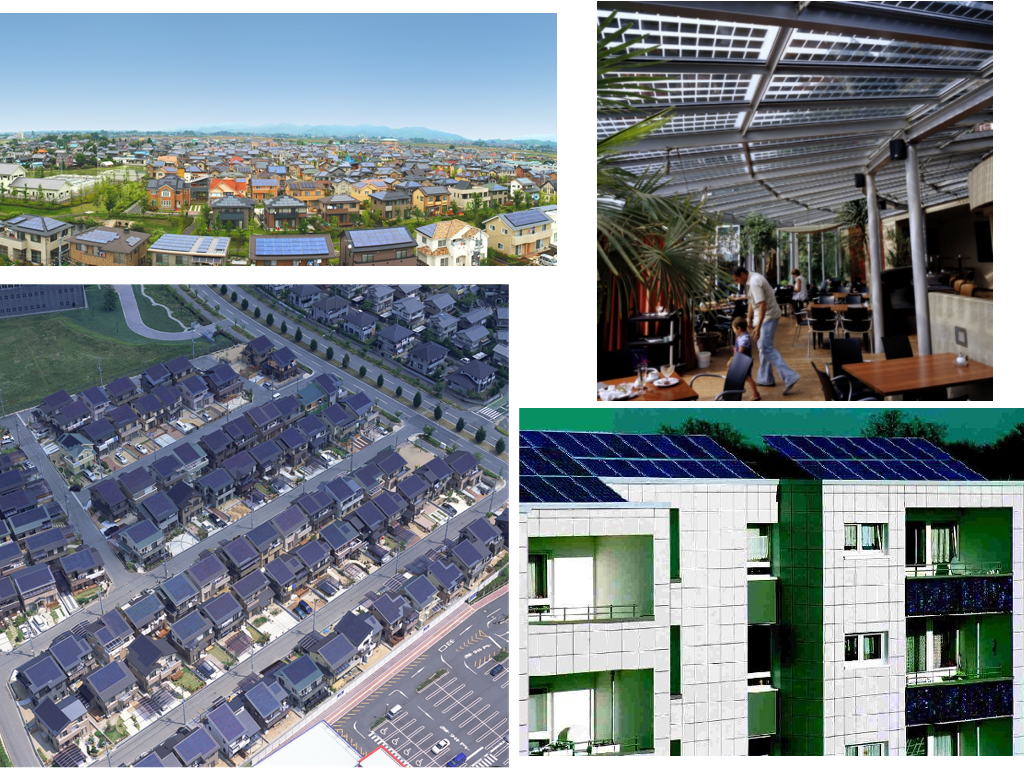
\includegraphics[height=0.5\textheight]{../figs/PVUrban.png}
\end{center}
\end{frame}


\begin{frame}[label={sec:orgf7ec604}]{From Horizontal to Inclined}
\begin{center}
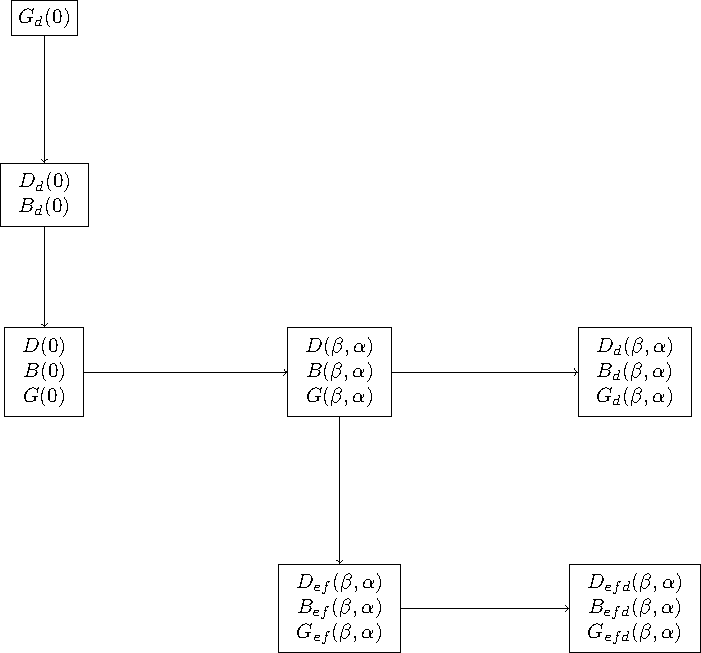
\includegraphics[width=.9\linewidth]{../figs/ProcedimientoCalculoRadiacionInclinada.pdf}
\end{center}
\end{frame}



\section{Solar Geometry}
\label{sec:org4990f96}

\begin{frame}[label={sec:orga3e4acf}]{Apparent Sun movement}
\begin{center}
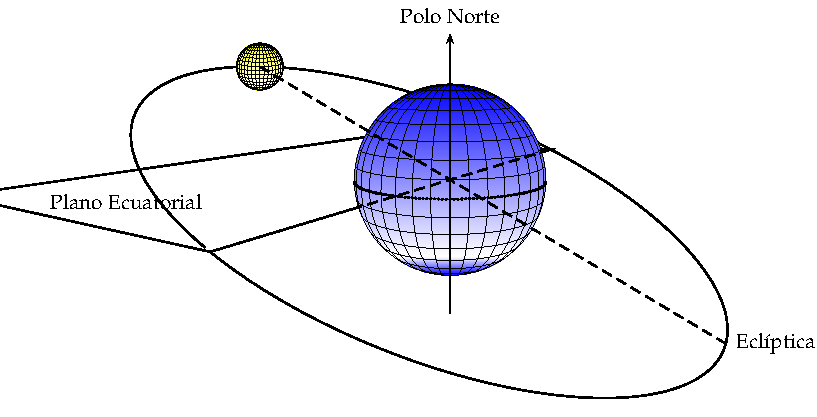
\includegraphics[width=.9\linewidth]{../figs/SoldesdeTierra.pdf}
\end{center}


\begin{block}{Declination Angle, \(\delta\)}
\begin{itemize}
\item Angle between the equatorial plane, and the line from the Sun to the center of the Earth.
\end{itemize}
\[
\delta=23.45\degree\cdot\sin(\frac{2\pi\cdot(d_{n}+284)}{365})
\]
\end{block}
\end{frame}

\begin{frame}[label={sec:org0be8bff}]{Declination Angle and Seasons}
\begin{itemize}
\item June solstice: \(\delta_{max}\)
\item December solstice: \(\delta_{min}\)
\item Equinoxes: \(\delta = 0\)
\end{itemize}

\begin{center}
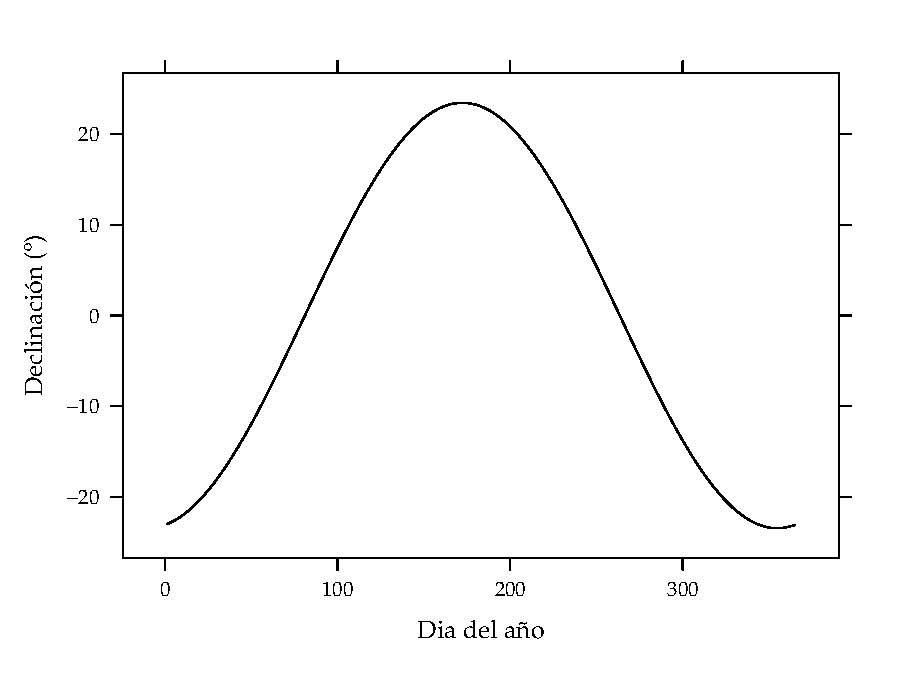
\includegraphics[width=.9\linewidth]{../figs/Declinacion.pdf}
\end{center}
\end{frame}

\begin{frame}[label={sec:org30ce218}]{Solar Hour Angle}
\begin{itemize}
\item \(w\), difference between the current instant and the noon or midday (\(w = 0\)).
\begin{itemize}
\item (Hours) \(-12, -11, -10, \dots, -1, \textbf{0}, 1, \dots, 10, 11, 12\)
\item 1h = 15º (\(24\text{h} = 2\pi \text{ radians} = 360\)).
\end{itemize}

\item Sunrise (\(w_s < 0\)):
\end{itemize}
\[
\cos(\omega_{s}) = -\tan(\delta)\tan(\phi)
\]

\begin{itemize}
\item Day length, \(|2 \cdot \omega_s|\), depends on the \alert{latitude}, \(\phi\), and on the \alert{day of year}.
\end{itemize}
\end{frame}

\begin{frame}[plain,label={sec:org153f8e2}]{Zenith Angle}
\[
\cos(\theta_{z}) = \cos(\delta) \cos(\omega) \cos(\phi) + \sin(\delta) \sin(\phi)
\]


\begin{columns}
\begin{column}{0.55\columnwidth}
\begin{itemize}
\item \(\theta_z\), angle between the Sun and the zenith (vertical in a particular location).
\item Depends on \(d_n\), \(\omega\), and \(\phi\).
\end{itemize}
\end{column}
\begin{column}{0.8\columnwidth}
\begin{center}
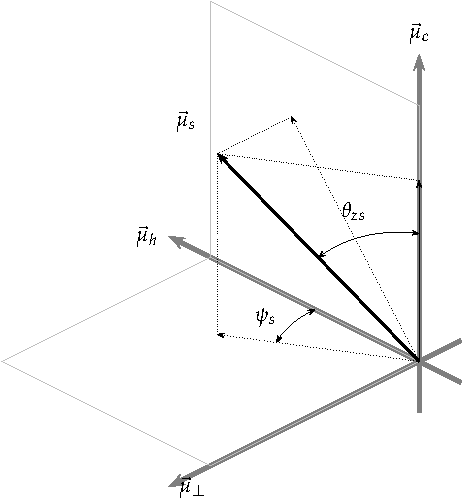
\includegraphics[width=.9\linewidth]{../figs/SistemaCoordenadasLocal-crop.pdf}
\end{center}
\end{column}
\end{columns}
\end{frame}

\begin{frame}[plain,label={sec:orgb228172}]{Azimuth Angle}
\[
  \cos(\psi_{s}) = \mathrm{sign}(\phi) \cdot \frac{\cos(\delta) \cos(\omega) \sin(\phi) - \cos(\phi) \sin(\delta)} {\sin(\theta_{z})}
\]

\begin{columns}
\begin{column}{0.55\columnwidth}
\begin{itemize}
\item \(\psi_s\), angle between the projection of Sun onto the horizontal plane and the noon.
\item Depends on \(d_n\), \(\omega\), and \(\phi\).
\end{itemize}
\end{column}

\begin{column}{0.75\columnwidth}
\begin{center}
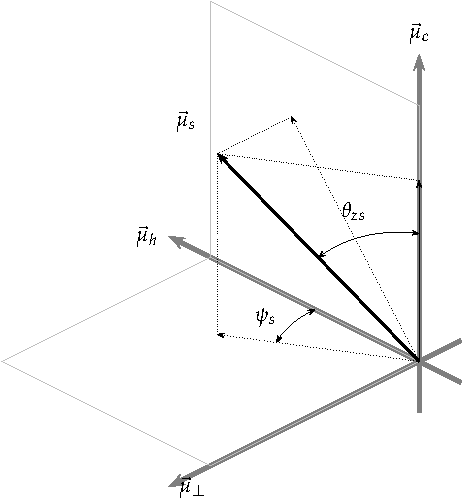
\includegraphics[width=.9\linewidth]{../figs/SistemaCoordenadasLocal-crop.pdf}
\end{center}
\end{column}
\end{columns}
\end{frame}

\begin{frame}[label={sec:org7c05e06}]{Sun Trajectory (\(40\degree S\))}
\begin{center}
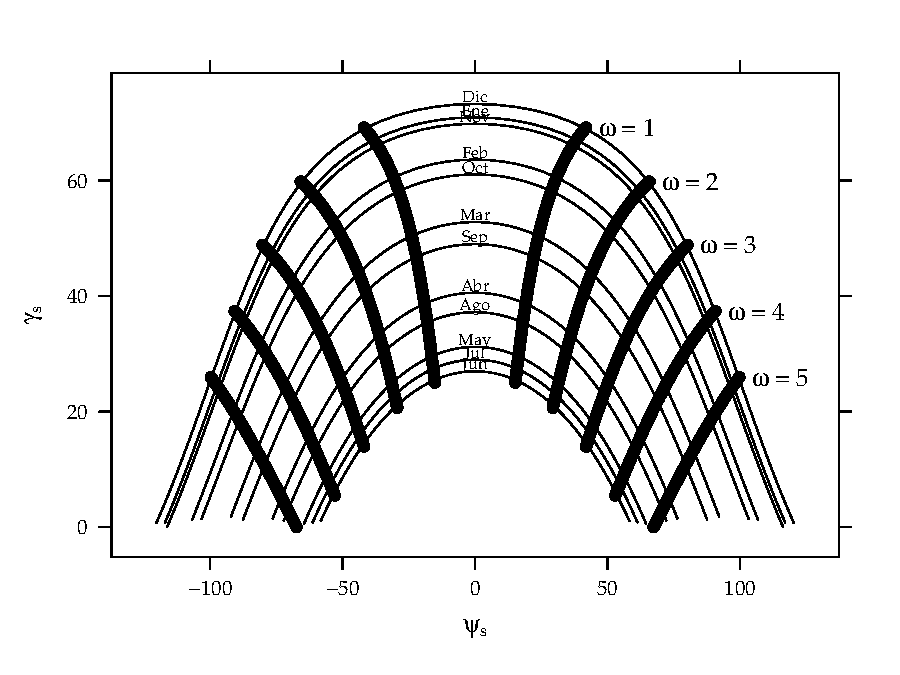
\includegraphics[width=.9\linewidth]{../figs/TrayectoriaSolar40S.pdf}
\end{center}
\end{frame}


\begin{frame}[label={sec:org56c95be}]{Extraterrestrial Irradiation}
\begin{itemize}
\item Solar radiation incident on a horizontal plane at top of the atmosphere.
\item Depends on the latitude and day of the year.
\end{itemize}

\begin{center}
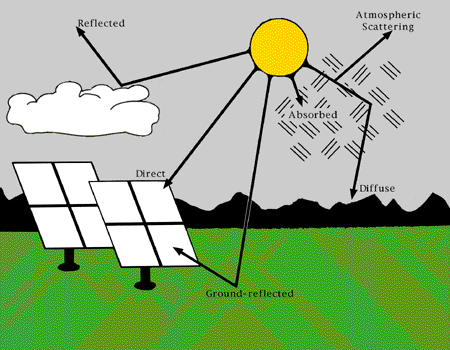
\includegraphics[height=0.5\textheight]{../figs/SolarRadiationComponents_NREL.png}
\end{center}
\end{frame}


\begin{frame}[label={sec:org6a18b3c}]{Extraterrestrial Irradiation}
\begin{itemize}
\item \(B_{0d}(0)=-\frac{24}{\pi}B_{0}\epsilon_{0}\cdot(\omega_{s}\sin\phi\sin\delta+\cos\delta\cos\phi\sin\omega_{s})\)
\begin{itemize}
\item \(\omega_{s}\) in radians
\item \(B_0 \simeq \SI{1367}{\watt\per\meter\squared}\) (Solar Constant)
\item Eccentricity correction factor, \(\epsilon_0 = 1+0,033\cdot\cos(2\pi d_n/365)\)
\end{itemize}
\end{itemize}
\end{frame}

\section{Angle of Incidence}
\label{sec:org31e47b1}
\begin{frame}[label={sec:orgd83984b}]{Definitions}
\begin{itemize}
\item \(\theta_s\), Angle of Incidence (AOI), angle between the solar rays and the line perpendicular to the generator surface
\item \(\alpha\): Orientation of the generator (0º when oriented to the noon)
\item \(\beta\): Inclination of the generator.
\end{itemize}
\end{frame}

\begin{frame}[label={sec:org582b081}]{Fixed System}
\begin{center}
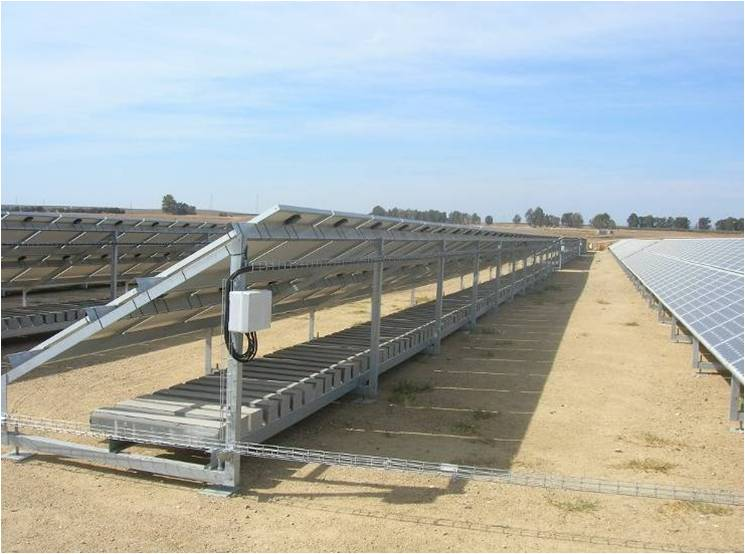
\includegraphics[width=.9\linewidth]{../figs/EstructuraEstaticaSuelo.jpg}
\end{center}
\end{frame}

\begin{frame}[plain,label={sec:org4e93c11}]{Fixed System}
\begin{itemize}
\item If \(\alpha=0\)
\end{itemize}
\[
\cos(\theta_{s}) = \cos(\delta)\cos(\omega)\cos(\beta-|\phi|)- \mathrm{sign}(\phi)\cdot\sin(\delta)\sin(\beta-|\phi|)
\]

\begin{center}
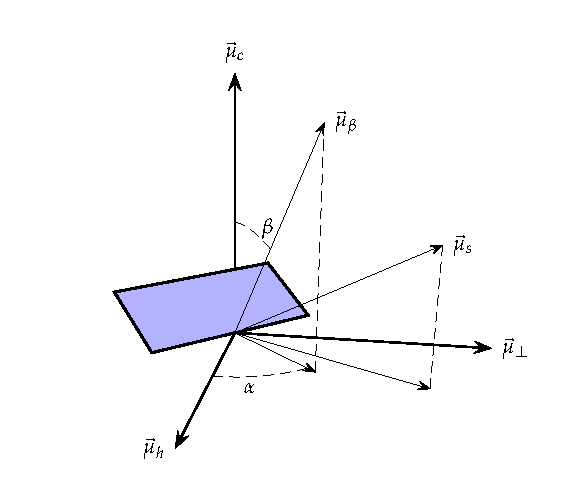
\includegraphics[height=0.6\textheight]{../figs/AngulosSistemaEstatico.pdf}
\end{center}

\begin{itemize}
\item Optimum Inclination \(\beta_{opt} \simeq |\phi| - 10º\).
\end{itemize}
\end{frame}

\begin{frame}[label={sec:orgf6e782d}]{Tracking System (1x axis, horizontal N-S)}
\begin{center}
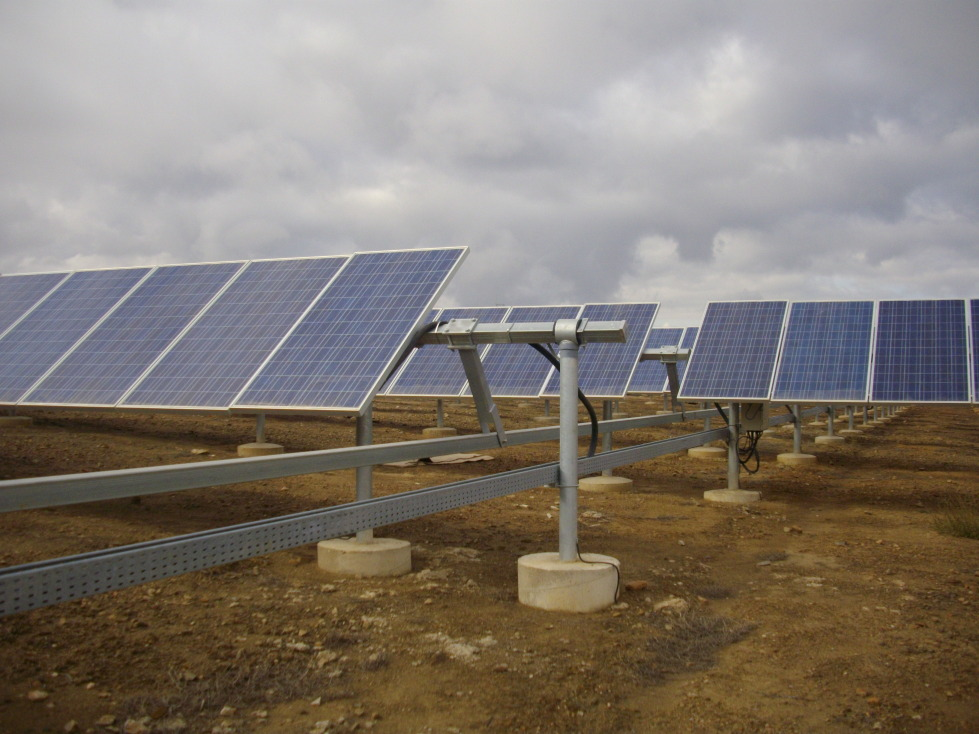
\includegraphics[width=.9\linewidth]{../figs/SeguidorEjeHorizontal.jpg}
\end{center}
\end{frame}


\begin{frame}[plain,label={sec:orgff3f2e9}]{Tracking System (1x axis, horizontal N-S)}
\[\cos(\theta_{s})=\cos(\delta)\sqrt{\sin^{2}(\omega)+\left(\cos(\omega)\cos(\phi)+\tan(\delta)\sin(\phi)\right)^{2}}\]

\begin{center}
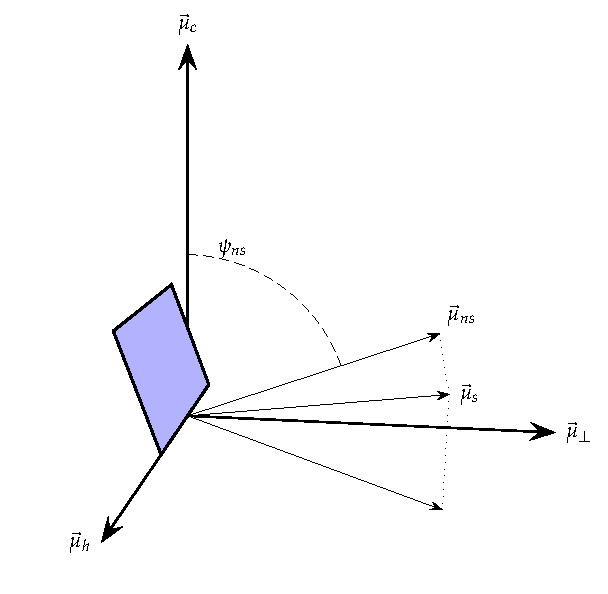
\includegraphics[height=0.6\textheight]{../figs/AngulosSistemaHorizontalNS.pdf}
\end{center}
\end{frame}



\begin{frame}[label={sec:org4a4893e}]{Tracking System (2x axis)}
\begin{center}
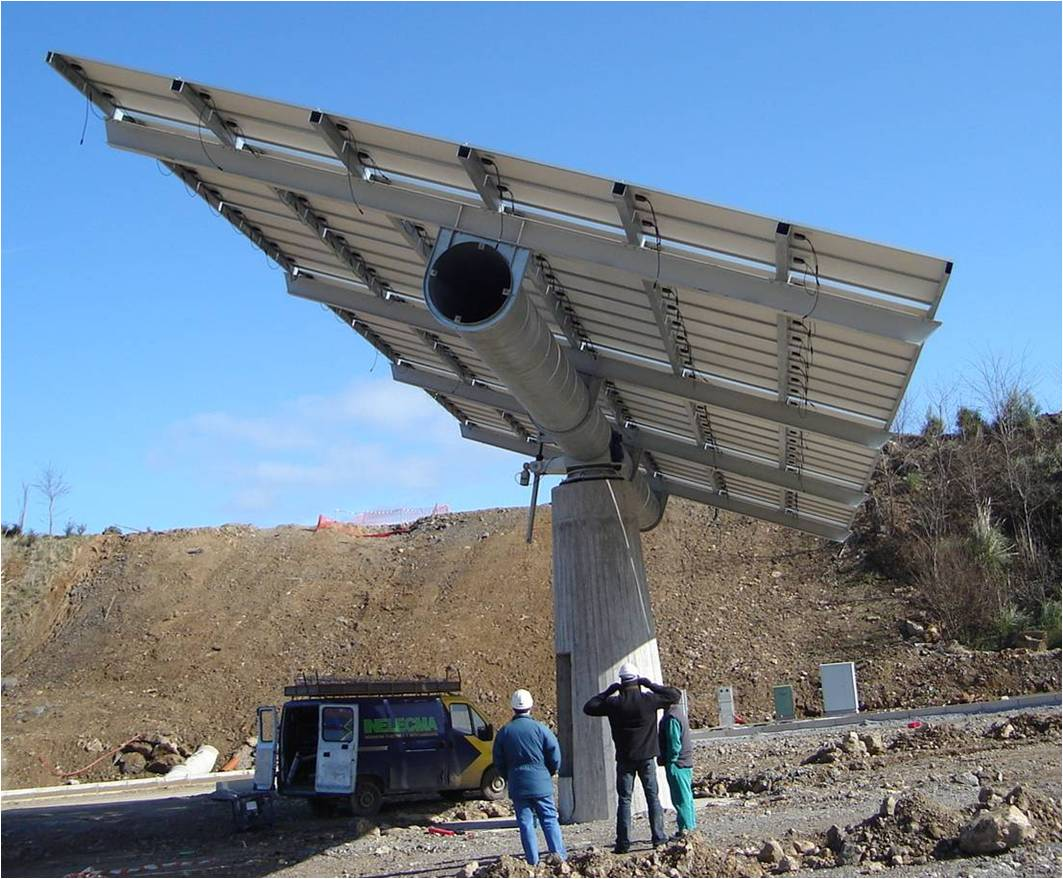
\includegraphics[width=.9\linewidth]{../figs/SeguidorReocin.jpg}
\end{center}
\end{frame}

\begin{frame}[plain,label={sec:org8193aea}]{Tracking System (2x axis)}
\begin{center}
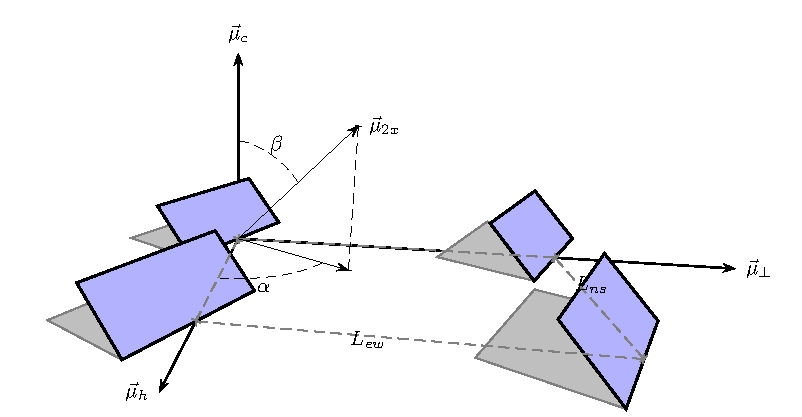
\includegraphics[width=.9\linewidth]{../figs/Sombra2X.pdf}
\end{center}


\begin{align*}
  \beta &= \theta_{z}\\
  \alpha &= \psi_{s}\\
  \cos(\theta_{s}) &= 1
\end{align*}
\end{frame}




\section{Transposition Procedure}
\label{sec:orgb497e40}

\begin{frame}[label={sec:org17bc151}]{Transposition Procedure}
\begin{center}
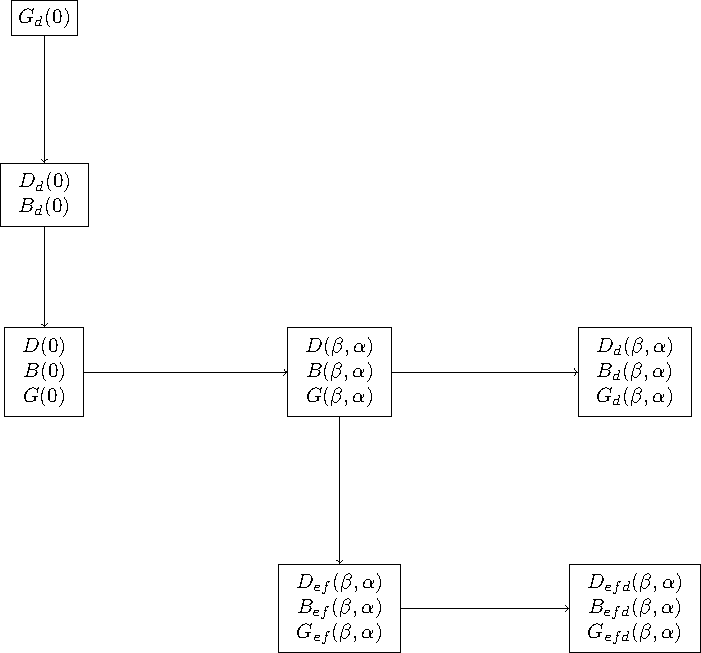
\includegraphics[width=.9\linewidth]{../figs/ProcedimientoCalculoRadiacionInclinada.pdf}
\end{center}
\end{frame}


\begin{frame}[label={sec:org0a42ebf}]{Extract Diffuse and Beam Components}
\begin{block}{Clearness Index}
\begin{itemize}
\item \(K_{Td} = G_{d}(0)/B_{0d}(0)\)
\end{itemize}
\end{block}

\begin{block}{Diffuse Fraction}
\begin{itemize}
\item \(F_{Dd}=\frac{D_d(0)}{G_d(0)}\)
\end{itemize}
\end{block}

\begin{block}{Model}
\begin{itemize}
\item Monthly values: \[F_{Dm}=1-1.13\cdot K_{Tm}\]

\item Daily values:
\end{itemize}
{\scriptsize \[
F_{Dd} = \begin{cases}
  0.99 & K_{Td} \leq 0.17\\
  1.188 - 2.272 \cdot K_{Td} + 9.473 \cdot K_{Td}^{2} - 21.856 \cdot K_{Td}^{3} + 14.648 \cdot K_{Td}^{4} & K_{Td} > 0.17
\end{cases}
\]
}
{\scriptsize \par}
\end{block}
\end{frame}


\begin{frame}[label={sec:orga107656}]{Example}
Let's \(G_{d,m}(0) = \SI{3150}{\watthour\per\meter\squared}\) in a month with \(B_{0,dm}(0) = \SI{4320}{\watthour\per\meter\squared}\). Thus:

\begin{itemize}
\item \(K_{Tm}=\frac{3150}{4320}=0.73\)

\item \(F_{Dm}=1-1.13\cdot0.73=0.175\)

\item \(D_{d,m}(0)=0.175\cdot3150=\SI{551.6}{\watthour\per\meter\squared}\)

\item \(B_{d,m}(0)=3150-551.6=\SI{2598,4}{\watthour\per\meter\squared}\)
\end{itemize}
\end{frame}

\begin{frame}[label={sec:org1b2f39d}]{Intradaily profile}
\begin{block}{Estimate irradiance from irradiation}
\begin{align*}
  D(0) &= r_D \cdot D_d(0)\\
  G(0) &= r_G \cdot G_d(0)\\
  B(0) &= G(0) - D(0)
\end{align*}

\begin{align*}
  r_{D} &= \frac{\pi}{T}\cdot\frac{\cos(\omega)-\cos(\omega_{s})}{\omega_{s}\cdot\cos(\omega_{s})-\sin(\omega_{s})}\\
  r_{G} &= r_{D}\cdot(a+b\cdot\cos(\omega))\\
  a &= 0.409-0.5016\cdot\sin(\omega_{s}+\frac{\pi}{3})\\
  b &=0.6609+0.4767\cdot\sin(\omega_{s}+\frac{\pi}{3})
\end{align*}
\end{block}
\end{frame}
\begin{frame}[label={sec:orgb8c5c56}]{Transposition to the Plane of Generator}
\begin{itemize}
\item Beam radiation
\end{itemize}

\[B(\alpha,\beta)=B(0)\cdot\frac{\max(0,\cos(\theta_{s}))}{\cos(\theta_{zs})}\]

\begin{itemize}
\item Diffuse Radiation (isotropic model)
\end{itemize}

\[D(\alpha,\beta)=D(0)\cdot\frac{1+\cos(\beta)}{2}\]

\begin{itemize}
\item Albedo
\end{itemize}

\[R(\beta,\alpha)=\rho\cdot G(0)\cdot\frac{1-\cos(\beta)}{2}\]

\[\rho=0.2\]

\begin{itemize}
\item Global
\end{itemize}
\[G(\alpha, \beta) = B(\alpha, \beta) + D(\alpha, \beta) + R(\alpha, \beta)\]
\end{frame}
\begin{frame}[label={sec:orgf50692a}]{Back to daily values}
\begin{block}{Daily values are the sum of hourly values in a day}
\begin{align*}
  G_d(\alpha, \beta) &= \sum_d G(\alpha, \beta)\\
  D_d(\alpha, \beta) &= \sum_d D(\alpha, \beta)\\
  B_d(\alpha, \beta) &= \sum_d B(\alpha, \beta)\\
\end{align*}
\end{block}
\end{frame}
\end{document}